\documentclass[conference]{IEEEtran}
\usepackage{mathptmx}
\usepackage{amsmath,amssymb,booktabs,cite,url}
\usepackage{tikz,pgfplots}
\pgfplotsset{compat=1.18}
\usepackage[hidelinks]{hyperref}
\setlength{\emergencystretch}{2em}
\title{Jevlet: A Shared Encoder for Typed Text Decisions with Expanded Question Validation}
\makeatletter
\newcommand{\linebreakand}{\end{@IEEEauthorhalign}\hfill\mbox{}\par\vspace{1em}\mbox{}\hfill\begin{@IEEEauthorhalign}}
\makeatother
\author{
\IEEEauthorblockN{\normalfont Hitanshu Gala}
\IEEEauthorblockA{\textit{Department of Information Technology}\\
\textit{Dwarkadas Jivanlal Sanghvi}\\
\textit{College of Engineering}\\
Mumbai, India}
\and
\IEEEauthorblockN{\normalfont Jay Dalvi}
\IEEEauthorblockA{\textit{Department of Information Technology}\\
\textit{Dwarkadas Jivanlal Sanghvi}\\
\textit{College of Engineering}\\
Mumbai, India}
\linebreakand
\IEEEauthorblockN{\normalfont Satishkumar Varma}
\IEEEauthorblockA{\textit{Department of Information Technology}\\
\textit{Dwarkadas Jivanlal Sanghvi}\\
\textit{College of Engineering}\\
Mumbai, India}
\and
\IEEEauthorblockN{\normalfont Richa Sharma}
\IEEEauthorblockA{\textit{Department of Information Technology}\\
\textit{Dwarkadas Jivanlal Sanghvi}\\
\textit{College of Engineering}\\
Mumbai, India}
}
\begin{document}
\maketitle
\begin{abstract}
Jevlet is designed as a shared DistilBERT encoder with typed choice, five-level sentiment, and binary heads. BANKING77 and SST-5 supply supervised labels. This stage documents the literature, problem statement, source data, preprocessing, mathematical model, and marker-based system architecture.
\end{abstract}
\begin{IEEEkeywords}
\bfseries
Jevlet , shared encoder , typed text decisions , multi-task learning , sentiment analysis , probability calibration
\end{IEEEkeywords}


\section{Introduction}
A banking support system may need to classify a message, decide whether it concerns a particular issue, and attach a confidence value to each answer. A review-analysis system may instead require a sentiment level from one to five. In both cases, the downstream application expects a small, structured answer space. Returning a typed value and its probability distribution makes that expectation explicit.

Jevlet uses a shared DistilBERT encoder and three task-specific heads to answer these bounded questions. A request contains a context and one to three questions. Each question specifies whether its answer is an option, a five-level score, or a boolean. The question block and context form one token sequence, so several questions can reuse an encoder pass. The implementation exposes confidence, an expected sentiment score, and the number of context tokens removed by truncation.

The purpose of this work is to explain and evaluate Jevlet as a practical model for typed decisions. Our contributions are the marker-conditioned multi-question architecture, an empirical sentiment-head revision, and a validation protocol that varies wording and banking candidate sets. We also measure calibration and inference cost. These contributions concern a supervised English banking-and-review workload; they do not establish unrestricted question answering or domain-independent sentiment understanding.

\section{Literature Review}
DistilBERT provides a compact pretrained transformer representation through knowledge distillation~\cite{distilbert}, building on bidirectional language representations studied in BERT~\cite{bert}. Jevlet fine-tunes this representation jointly with its typed heads rather than treating the encoder as a frozen feature extractor. Its engineering design draws on Laya's typed interface and marker scoring~\cite{laya}, but Jevlet implements its own heads and packed multi-question sequences.

Ordered sentiment levels motivate cumulative ordinal regression~\cite{coral}. However, a mathematically ordered distribution can still assign too little probability to intermediate classes under an argmax decoder. We therefore examine a categorical five-class head as a direct alternative. Temperature scaling~\cite{guo} and Brier error~\cite{brier} are used to evaluate probability quality separately from answer correctness.

\section{Methodology and System Architecture}
\subsection{Preprocessing and Request Packing}
The input is a context $x$ with questions $Q=\{q_1,\ldots,q_m\}$, where $1\leq m\leq3$. Each question has a unique identifier, a type, and nonempty text. Choice questions additionally supply two to ten distinct options. The packed representation is
\begin{equation}
[\mathrm{CLS}]\;B(Q)\;[\mathrm{SEP}]\;x\;[\mathrm{SEP}],
\end{equation}
where $B(Q)$ contains a \texttt{[Q]} marker before each question and a \texttt{[OPT]} marker before every choice option. Both markers are added to the tokenizer vocabulary and learned during fine-tuning.

The sequence has a 256-token budget. The question block is retained first, and the context is truncated only if necessary. An oversized question block that leaves no context room is rejected. Literal reserved-token strings in input text are removed before tokenization to prevent accidental extra markers. Padding masks hide unused sequence positions. Marker positions are recorded during packing so the output heads can gather the correct vectors.

\subsection{Shared Encoder and Marker Representations}
DistilBERT-base supplies six transformer layers, hidden dimension 768, and twelve attention heads. Self-attention contextualizes the question and option markers jointly with the text. If $H$ is the encoder output, Jevlet reads $h_{q_i}$ from the marker for question $i$ and $h_{o_{ij}}$ from the marker for its option $j$. The heads are linear projections of these vectors.

Several questions share the context tokens and the encoder computation. This is a concrete implementation property rather than evidence of general reasoning: the model learns from the task labels and question forms present during supervision. Packing also creates a tradeoff, because longer questions and option lists reduce the remaining context budget.


\begin{figure*}[t]
\centering
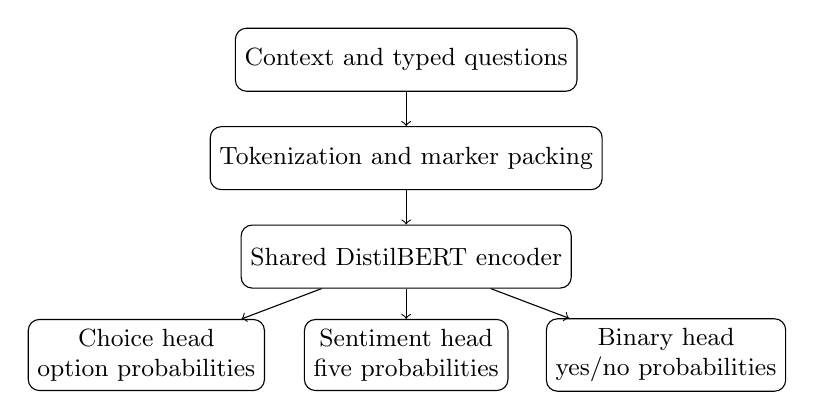
\begin{tikzpicture}[node distance=1.25cm, every node/.style={draw,rounded corners,align=center,font=\small,minimum height=0.8cm}]
\node (input) {Context and typed questions};
\node (tokens) [below of=input] {Tokenization and marker packing};
\node (encoder) [below of=tokens] {Shared DistilBERT encoder};
\node (choice) [below of=encoder,xshift=-3.3cm] {Choice head\\option probabilities};
\node (score) [below of=encoder] {Sentiment head\\five probabilities};
\node (binary) [below of=encoder,xshift=3.3cm] {Binary head\\yes/no probabilities};
\draw[->] (input)--(tokens); \draw[->] (tokens)--(encoder);
\draw[->] (encoder)--(choice); \draw[->] (encoder)--(score); \draw[->] (encoder)--(binary);
\end{tikzpicture}
\caption{Jevlet's system architecture. Marker representations feed typed heads after one packed encoder pass.}
\label{fig:architecture}
\end{figure*}

\subsection{Choice and Binary Heads}
The choice scorer maps every option representation to a scalar,
\begin{equation}
z_{ij}=w_c^\top h_{o_{ij}}+b_c,\qquad
p_{ij}=\frac{\exp(z_{ij}/T_c)}{\sum_{k\in O_i}\exp(z_{ik}/T_c)}.
\end{equation}
Only supplied options participate in the softmax. Unused option slots are masked, and the maximum-probability option is returned as the typed answer. Its probability is relative to the current shortlist.

The binary head reads a question marker and produces
\begin{equation}
p_i(\mathrm{yes})=\sigma((w_b^\top h_{q_i}+b_b)/T_b).
\end{equation}
The no probability is its complement. The predicted answer is a boolean, and confidence is the probability of that predicted answer. Training predicates refer to known banking intents; the interface alone does not establish understanding of arbitrary predicates.

\subsection{Five-Level Sentiment Head}
The categorical head maps the sentiment question marker to five logits:
\begin{equation}
\boldsymbol{p}_i=\operatorname{softmax}((W_s h_{q_i}+b_s)/T_s).
\end{equation}
The levels correspond to very negative, negative, neutral, positive, and very positive review sentiment. The discrete answer is $1+\arg\max_j p_{ij}$, and the expected score is $\sum_{j=1}^{5}j p_{ij}$. The latter retains uncertainty that a single discrete level hides.

The original head instead learns a scalar $s$ and four ordered thresholds $\beta_1<\cdots<\beta_4$, using softplus increments to preserve order. With $u_k=\sigma((s-\beta_k)/T_s)$, the probabilities are $(1-u_1,u_1-u_2,u_2-u_3,u_3-u_4,u_4)$. Narrow threshold spacing can leave intermediate levels weakly represented under argmax. The categorical revision changes both the parameterization and the supervised sentiment loss, so their effects cannot be separated by this ablation alone.

\section{Dataset Selection and Preprocessing}
\subsection{Dataset Description and Supervision}
BANKING77 supplies 77 banking intent labels~\cite{banking}. SST-5 supplies English review sentiment labels~\cite{sst}. Contexts are partitioned before questions are derived. Case-folded, whitespace-normalized duplicate contexts are removed with test taking precedence; the manifest records 15 within-split and 11 cross-split removals. Retained counts appear in Table~\ref{tab:data}.

\begin{table}[t]
\caption{Unique source texts; unchanged across the Jevlet experiments}
\label{tab:data}\centering
\begin{tabular}{lrrr}\toprule
Partition & Banking & Reviews & Total\\\midrule
Training & 7,993 & 8,531 & 16,524\\
Validation & 999 & 550 & 1,549\\
Calibration & 1,000 & 550 & 1,550\\
Test & 3,079 & 2,210 & 5,289\\\bottomrule
\end{tabular}\end{table}

Banking choice questions include the true intent and one to nine sampled alternatives. Yes/no labels are sampled positive with probability 0.5. In packed requests, queried labels occur among the supplied options, removing a simple option-presence shortcut. Training samples choice-only, binary-only, paired, and three-question recipes, with deterministic epoch-wise variation in candidates and question order. The fixed canonical evaluation request has one choice and two binary questions per banking text, or one sentiment question per review.

The choice task evaluates a shortlist containing the correct label, not retrieval over all 77 labels. Binary prevalence is approximately balanced by construction. Banking texts do not supply sentiment labels, and review texts do not supply banking intent labels.


\section{Conclusion}
The dataset, preprocessing pipeline, and shared DistilBERT architecture were selected for Jevlet. Typed heads provide a practical design for intent, sentiment, and binary decisions.
\begin{thebibliography}{10}
\bibitem{distilbert}V. Sanh, L. Debut, J. Chaumond, and T. Wolf, ``DistilBERT, a distilled version of BERT: Smaller, faster, cheaper and lighter,'' \emph{arXiv preprint arXiv:1910.01108}, 2019. [Online]. Available: \url{https://arxiv.org/abs/1910.01108}
\bibitem{bert}J. Devlin, M.-W. Chang, K. Lee, and K. Toutanova, ``BERT: Pre-training of deep bidirectional transformers for language understanding,'' in \emph{Proc. NAACL-HLT}, 2019, pp. 4171--4186, doi: 10.18653/v1/N19-1423.
\bibitem{laya}N. Mukkunnoth and Convai Innovations, ``Laya: Non-autoregressive System 1 decision engine,'' GitHub repository. Accessed: Oct. 11, 2026. [Online]. Available: \url{https://github.com/NandhaKishorM/laya}
\bibitem{coral}W. Cao, V. Mirjalili, and S. Raschka, ``Rank consistent ordinal regression for neural networks with application to age estimation,'' \emph{Pattern Recognition Letters}, vol. 140, pp. 325--331, 2020. [Online]. Available: \url{https://arxiv.org/abs/1901.07884}
\bibitem{guo}C. Guo, G. Pleiss, Y. Sun, and K. Q. Weinberger, ``On calibration of modern neural networks,'' in \emph{Proc. 34th Int. Conf. Machine Learning}, vol. 70, 2017, pp. 1321--1330. [Online]. Available: \url{https://proceedings.mlr.press/v70/guo17a.html}
\bibitem{brier}G. W. Brier, ``Verification of forecasts expressed in terms of probability,'' \emph{Monthly Weather Review}, vol. 78, no. 1, pp. 1--3, 1950.
\bibitem{banking}I. Casanueva, T. Temcinas, D. Gerz, M. Henderson, and I. Vuli\'{c}, ``Efficient intent detection with dual sentence encoders,'' in \emph{Proc. 2nd Workshop on Natural Language Processing for Conversational AI}, 2020, pp. 38--45, doi: 10.18653/v1/2020.nlp4convai-1.5.
\bibitem{sst}R. Socher, A. Perelygin, J. Wu, J. Chuang, C. D. Manning, A. Ng, and C. Potts, ``Recursive deep models for semantic compositionality over a sentiment treebank,'' in \emph{Proc. EMNLP}, 2013, pp. 1631--1642. [Online]. Available: \url{https://aclanthology.org/D13-1170/}
\end{thebibliography}
\end{document}
